\documentclass[dvisvgm,tikz]{standalone}
\usepackage{circuitikz}
\begin{document}
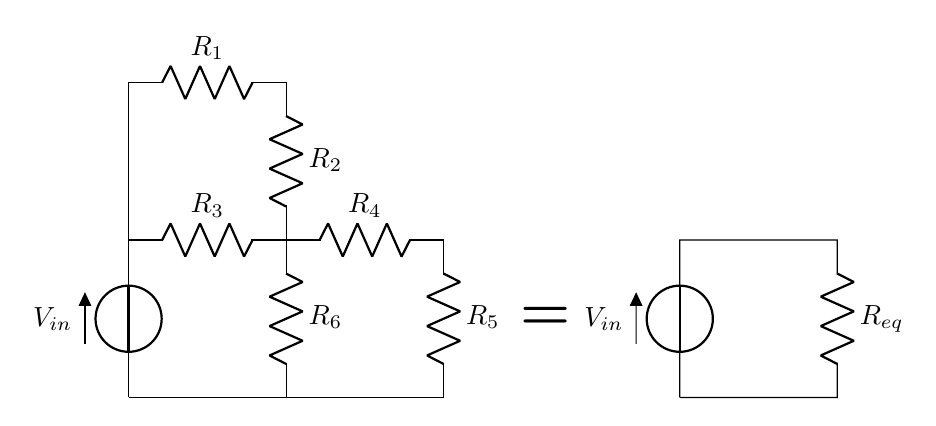
\begin{tikzpicture}
  \draw (0,-2)
  to[short] (0,0)
  to[R=$R_1$] (2,0)
  to[R=$R_2$] (2,-2);
  \draw (0,-4)
  to[V,v=$V_{in}$,invert] (0,-2)
  to[R=$R_3$] (2,-2)
  to[R=$R_4$] (4,-2)
  to[R=$R_5$] (4,-4)
  to[short] (0,-4);
  \draw (2,-2)
  to[R=$R_6$] (2,-4);
  \node at (5.3,-3) {\textbf{\huge =}};
  \draw (7,-4)
  to[V,v=$V_{in}$,invert] (7,-2)
  to[short] (9,-2)
  to[R=$R_{eq}$] (9,-4)
  to[short] (7,-4);
\end{tikzpicture}
\end{document}
